\documentclass[a4paper,14pt]{extarticle}
\usepackage[utf8]{inputenc}
\usepackage[russian]{babel}
\usepackage[a4paper, mag=1000, left=2.5cm, right=1cm, top=2cm, bottom=2cm, headsep=0.7cm, footskip=0cm]{geometry}

\title{Анализ и визуализация плагиата исходного кода в практических курсах по программированию. Source code plagiarism analysis and visualization for programming courses.}
\author{Андрей Цибин, бакалавр, tsibin.andr@gmail.com\\Евгений Ефимчик, к.т.н, eugene.efimchick@gmail.com}
\date{Университет ИТМО, Май 2020}

\usepackage{natbib}
\usepackage{graphicx}
\usepackage{url}
\usepackage{amsmath}
\usepackage{booktabs}

\begin{document}

\maketitle

\begin{abstract}

Проблема недобросовестного заимствования в академической среде по-прежнему
является актуальной. Недобросовестные заимствования, или плагиат, встречаются сегодня в различных формах академической активности, начиная от семестровых работ студентов и заканчивая диссертациями ученых. Развитие коммуникаций, глобальный характер взаимодействия привели к широкой доступности материалов, которые легко скопировать. Это приводит к тому, что студентам становится проще найти решение, чем его составить. Отдельной проблемой
являются недобросовестные заимствование в работах обучающихся учебных заведений, которые они выполняют в рамках практических курсов по программированию. Как и в случае с текстом, выявлять плагиат вручную является возможным только в самых небольших подвыборках данных. К счастью, на сегодняшний день существует довольно большое количество систем, позволяющих
автоматизировано выявлять сходство исходного кода. Более того, существуют
средства, позволяющие агрегировать результаты поиска плагиата несколькими
различными системами, что также увеличивает вероятность обнаружения случаев недобросовестного заимствования. При этом, применение данных средств
по-прежнему не так широко распространено в образовательных учреждениях.
В настоящей статье приводится описание процесса анализа плагиата, построенного для использования в рамках практических курсов по программированию, а также рассмотрен инструмент интерактивной графовой визуализации результатов анализа плагиата.

Ключевые слова: Плагиат, Академическая недобросовестность, Автоматизация, Заимствования, Практические курсы.

\end{abstract}

\section{Введение}

Задача выявления плагиата применительно к практическим курсам по программированию становится с каждым годом все более актуальной \citep{plagiarismEpidemic}. Открытые онлайн-курсы по программированию, зачастую, имеют целые базы открытых решений. Чаще всего они публикуются в рамках коммуникации обучающихся,  выполнивших задания, однако недобросовестно использовать их может кто угодно. Бороться с публикацией решений не представляется возможным, поскольку решения заданий могут публиковаться на различных платформах. По этой причине бороться необходимо с заимствованиями решений, т.е. искать плагиат в работах обучающихся. В настоящий момент контроль добросовестности становится в большей степени необходимостью, чем второстепенной возможностью \citep{sciencePlagiarismPaper}. Кроме того, как показывают некоторые исследования, существование механизма анализа плагиата в образовательном процессе повышает общее качество обучения навыкам программирования \citep{plagCheckEffect}\citep{plagInterventionEffect}.

Современные тенденции возрастания доли самостоятельной работы обучающихся, студенческой мобильности и развития дистанционных технологий обучения особенно остро ставят проблему организации практической работы в гибком, асинхронном режиме. Для решения этой проблемы в дисциплинах, связанных с практикой программирования, в Университете ИТМО была создана образовательная система Flaxo\footnote{Образовательная платформа Flaxo. \url{https://github.com/tcibinan/flaxo}} для организации и проведения практических курсов по программированию. Система воплощает идею многофакторного автоматизированного анализа и оценивания работ обучающихся, включающую критерии оценки соответствия спецификации с помощью функционального тестирования, формальной оценки качества кода с помощью инструментов статического анализа и выявления заимствований между решениями. Причем более актуальной задачей является поиск заимствований среди обучающихся одного практического курса, поскольку работа с системой направлена на взаимодействие с относительно небольшими группами обучающихся (до 100 человек), выполняющими ряд специализированных заданий.

Важно отметить, что работа с системой Flaxo направлена на взаимодействие с относительно небольшими группами обучающихся (до 100 человек) и со специализированными заданиями. Поэтому   более актуальна проблема поиска заимствований среди обучающихся одного практического курса, поскольку она направлена на работу с относительно небольшими группами (до 100 обучающихся) и с заданиями (... специализированными, нетривиальными, повышенного объема, ...).

Система была разработана в рамках бакалаврской выпускной квалификационной работы \citep{flaxoThesis}\citep{flaxoKmu}, и с начала учебного года 2018-2019 постепенно внедряется в дисциплинах образовательной программы "Нейротехнологии и программирование".

Далее в статье описаны техническое решение для модуля анализа плагиата указанной выше системы и формы визуализации его результатов.

\section{Схема хранения заданий и решений}

Концепция образовательной платформы Flaxo включала хранение всех заданий и решений обучающихся в репозиториях системы контроля версий. Так, задания представляют собой ветки репозитория преподавателя, а решения - запросы на слияние, создаваемые обучающимися к этим веткам. В текущем версии системы реализована поддержка системы версионирования Git\footnote{Распределенная система версионирования Git. \url{https://git-scm.com/}} и платформы GitHub\footnote{Платформа разработки GitHub. \url{https://github.com/}}, которая на сегодняшний день является одной из самых популярных систем для open-source проектов.

Для того чтобы провести анализ существующих решений, необходимо сначала собрать весь исходный код: файлы, представленные преподавателем, которые называются \textit{базовыми}, а также все файлы, измененные или созданные обучающимися. Учитывая, что репозитории с заданиями и решениями помимо исходного кода могут содержать множество других файлов, например, скрипты системы сборки проекта или документацию, необходимо перед выгрузкой заданий и решений фильтровать содержания репозиториев по расширениям файлов. Также загружаемые файлы должны быть сгруппированы по обучающемуся, который их создал или изменил, чтобы дальнейший анализ мог различать автора того или иного фрагмента кода. 

\section{Инструменты анализа заимствований}

Одна из основных задач, возникающая при попытке внедрения системы анализа плагиата это, безусловно, подбор инструментов выявления заимствований программного кода. В \citep{plagiarismToolsSurvey} приведен обзор значительного количества существующих инструментов. Они различаются механизмом анализа плагиата, форматами входных и выходных данных, скоростью обработки программного кода, а также количеством поддерживаемых языков программирования. Помимо прочего, существуют унифицированные подходы к анализу плагиата \citep{unifiedPlagiarismDetectionTool}\citep{gitplagThesis}, которые агрегируют результаты работы нескольких анализаторов и позволяют минимизировать число ложных срабатываний каждого в отдельности. Кроме того, в \citep{codeStyleDetectionTool},\citep{anotherPlagAnalysisTool},\citep{languageIndependentPlagiarismTool} описаны и другие средства анализа плагиата.

На основе проанализированной литературы и описаний существующих инструментов при разработке настоящего модуля анализа плагиата был выбран инструмент MOSS \citep{mossOriginalPaper}.

MOSS является бесплатным веб-сервисом поиска плагиата, поддерживающим поиск плагиата на 26 языках программирования. Сервис предоставляет Perl-скрипт в качестве клиентского приложения, который позволяет загружать файлы с исходным кодом и инициализировать анализ плагиата. Наряду с обычными файлами, MOSS использует упомянутое выше понятие базовых файлов. Под этим термином подразумеваются файлы, созданные преподавателем, строки которых должны быть проигнорированы при выявлении заимствованных фрагментов исходного кода.

Как было сказано выше, MOSS принимает на вход набор файлов для анализа, а на выходе генерирует набор HTML-страниц, которые содержат подробные отчеты по каждой паре решений, содержащих заимствованные коды. Отчет включает в себя количество и процент общих строчек всех файлов, а также таблицы с исходным кодом решений, включающие цветовое обозначение общих фрагментов кода.

Механизм поиска заимствований инструментом MOSS заключается в преобразовании исходного кода решений в наборы токенов и их фильтрации, составлению подгрупп цифровых отпечатков решений на основе выделенных токенов, а также непосредственного сравнения выбранных отпечатков отдельных решений. Предварительные преобразование исходного кода в токены и их фильтрация позволяют не учитывать при поиске заимствований неспецифичные части решений, как например, базовый код, комментарии, расстановку пробелов и переносов строк, имена переменных и методов. Кроме того, подход к выбору подгрупп цифровых отпечатков и их сравнению, используемый инструментом, позволяет находить заимствования с учетом базовых рефакторингов кода, как например, вынесение переменной или выделение метода.

Несмотря на все преимущества сервис MOSS обладает рядом недостатков. Во-первых, формат выходных данных HTML не пригоден для эффективной автоматической обработки, поэтому результаты анализа необходимо автоматически разбирать и преобразовывать в другой формат данных. Кроме того, сервис удаляет результаты анализа плагиата спустя 14 суток, в связи с чем результаты его работы требуется полностью выгружать до истечения этого срока.

Важно отметить, что архитектурно предусмотрена возможность замены используемого инструмент анализа заимствований. Таким образом, вместо используемого стороннего сервиса для поиска заимстований MOSS, могут быть также использованы и другие обозначенные выше инструменты, которые на текущий момент еще не поддерживаются.

\section{Представление результатов анализа заимствований}

\subsection{Индикация найденных заимствований}

Образовательная система Flaxo формирует сводные таблицы (Рис. \ref{fig:plagiarismIndication}) для отображения результатов автоматизированных проверок решений обучающихся. В качестве первичной индикации найденных заимствований система приводит в соответствие каждому решению пару показателей: количество найденных заимствований и максимальное значение процента общего кода среди всех найденных заимствований. Дополнительно, решения, показатель процента общего кода которых превышает некоторый заданный порог, например 80\%, выделяются красным цветом.

\begin{figure}[h!]
\centering
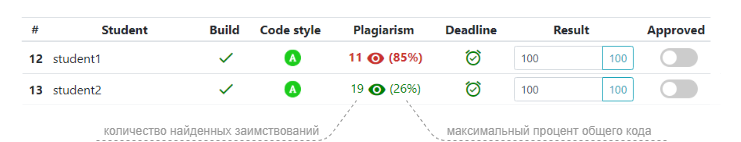
\includegraphics[width=1.0\textwidth]{plagiarism_indication.png}
\caption{Первичная индикация найденного плагиата}
\label{fig:plagiarismIndication}
\end{figure}

Описанный способ визуализации позволяет доступным образом указать преподавателю на работы, которые необходимо исследовать в первую очередь, а какие с меньшей вероятностью обладают недобросовестными заимствованиями. Тем не менее подобная система не позволяет визуализировать связи между работами, особенно, если одну работу скопировали несколько раз.

Действительно, механизм анализа плагиата предполагает попарное сравнение всех работ обучающихся, поэтому выявление небинарных зависимостей может оказаться непростой задачей. При этом, подобные зависимости, могут выявлять, например, группы недобросовестных обучающихся, которые делятся друг с другом своим исходным кодом. При этом, если похожие заимствования имеются более чем у двух людей, то это значительно уменьшает вероятность ложного срабатывания системы анализа плагиата.

\subsection{Графовая визуализация}

Таким образом, для определения связей между работами обучающихся, в том числе информации о том, кто у кого и сколько заимствовал, необходим инструмент, способный отображать общую картину связей между решениями.

Одним из возможных способов представления данных, позволяющим наблюдать подобные сложные зависимости, является графовая визуализация. На сегодняшний день существует несколько инструментов графовой визуализации результатов анализа плагиата \citep{plagiarismGraph}\citep{graphVisualizationCompetition}. Как показано в связанных статьях, использование графов для отображения результатов анализа плагиата наравне с гистограммами распределения процента заимствованного кода, повышает эффективность применения системы анализа плагиата в целом. Кроме того, использование наложенных графовых представлений нескольких заданий в практических курсах, позволяет значительно снизить число ложных срабатываний алгоритма анализа плагиата. При таком подходе становится возможным выявлять группы обучающихся, которые стабильно выделяются на фоне своих коллег и тем самым, вероятнее всего, действительно недобросовестно используют чужой исходный код.

Использование графов для отображения результатов анализа плагиата даже одного задания в отдельности, с точки зрения наглядности, имеет очевидные преимущества перед табличным представлением.

\subsubsection{Инструмент графовой визуализации}

Упомянутый выше инструмент визуализации плагиата делает большой шаг вперед к простоте интерпретации результатов анализа плагиата. Однако, он не позволяет динамически менять параметры, определяющие структуру графа, что ограничивает преподавателя в возможности наглядного рассмотрения зависимостей в различных перспективах и с отличающимся масштабом. По этой причине был создан инструмент\footnote{Инструмент интерактивной визуализации графов. \url{https://github.com/tcibinan/data2graph}} интерактивной визуализации графов.

Инструмент рассматривает обучающихся как вершины графа, а случаи заимствования как ребра графа, соединяющие двух различных обучающихся. В качестве веса ребра $w$ используется значение процента соответствующего заимствования, которое лежит в интервале $[0,100]$. Процент заимствования может составлять разную долю в исходном и скопированном решении. Тем не менее на практике разница составляет единицы процентов и для отображения выбирается наибольшее значение. Учитывая, что б\'{о}льшие веса соответствуют меньшим расстояниям между двумя решениями в пространстве всех возможных решений некоторой задачи, значения длин ребер $l$ должны быть тем меньше, чем больший вес им соответствует. При таком подходе на построенном графе можно визуально различать кластеры, каждый из которых определяет группу обучающихся, работы которых содержат значительно выделяющееся количество заимствований друг между другом. В случае отсутствия ярко выделенных кластеров, можно говорить о том, что примеров плагиата в работах найти не удалось или о том, что необходимо изменить параметры отображения графа.

В рамках проведения ряда практических курсов по программированию с использованием образовательной системы Flaxo было отмечено следующее явление: среднее значение процента общего кода всех найденных заимствований для каждого задания уникально и может значительно отличаться. При этом число подтвержденных случаев заимствований не всегда зависит от выявленного среднего значения процента общего кода.

В таблице \ref{tab:javaCourseStats} приведена статистика найденных заимствований для девяти заданий практического курса по изучению языка программирования Java. В частности, для каждого из заданий указаны число обучающихся, выполнивших задание, суммарное число отправленных ими решений, а также минимальное, максимальное и среднее значение процента общего кода среди всех найденных заимствований. В рамках исследования найденных заимствований в этом практическом курсе были подтверждены несколько случаев плагиата для части заданий. Можно заметить, что в приведенных данных для большинства заданий максимальные проценты общего кода заимствований не превышают 50\%, хотя некоторые из обнаруженных заимствований почти полностью копируют оригинальные решения. Такие заниженные показатели найденных заимствований вызваны большой долей базового кода, который не определяется как заимствование, но учитывается в общем количестве кода, относительно которого рассчитывается процент заимствований системой MOSS.

\begin{table}[htb]
    \centering
    \begin{tabular}{cccccc}
        \toprule
        № Задания & Кол-во обучающихся & Кол-во решений & Мин, \% & Макс, \% & Сред, \% \\
        \toprule
        1 & 18 & 52 & 1 & 16 & 5 \\
        \midrule
        2 & 17 & 49 & 1 & 33 & 8 \\
        \midrule
        3 & 17 & 49 & 1 & 28 & 7 \\
        \midrule
        4 & 17 & 76 & 1 & 27 & 6 \\
        \midrule
        5 & 17 & 67 & 5 & 77 & 25 \\
        \midrule
        6 & 17 & 42 & 1 & 13 & 4 \\
        \midrule
        7 & 17 & 44 & 1 & 41 & 7 \\
        \midrule
        8 & 15 & 38 & 3 & 50 & 15 \\
        \midrule
        9 & 15 & 28 & 2 & 38 & 11 \\
        \bottomrule
    \end{tabular}
    \caption{Статистика найденных заимствований курса по Java}
    \label{tab:javaCourseStats}
\end{table}

Одним из способов увеличения точности находимых заимствований является минимизация базового кода. В таблице \ref{tab:cppCourseStats} приведена статистика найденных заимствований другого практического курса, который направлен на изучение языка программирования C++. В связи со спецификой механизма автоматизированного тестирования решений в этом курсе, количество базового кода в нем сведено к минимуму. Как можно увидеть, величина максимального процента общего кода заимствований в этом курсе значительно выше, чем в курсе по Java, и для большинства заданий выше 80\%. Хочется отметить, что абсолютное большинство найденных заимствований с высоким процентом общего кода являются подтвержденными случаями плагиата.

\begin{table}[htb]
    \centering
    \begin{tabular}{cccccc}
        \toprule
        № Задания & Кол-во обучающихся & Кол-во решений & Мин, \% & Макс, \% & Сред, \% \\
        \toprule
        1 & 46 & 162 & 6 & 73 & 16 \\
        \midrule
        2 & 43 & 140 & 6 & 86 & 15 \\
        \midrule
        3 & 45 & 208 & 8 & 86 & 17 \\
        \midrule
        4 & 44 & 191 & 5 & 82 & 14 \\
        \midrule
        5 & 45 & 185 & 3 & 90 & 15 \\
        \midrule
        6 & 44 & 124 & 7 & 85 & 16 \\
        \midrule
        7 & 42 & 137 & 7 & 75 & 16 \\
        \midrule
        8 & 42 & 88 & 3 & 85 & 15 \\
        \midrule
        9 & 39 & 81 & 5 & 90 & 19 \\
        \midrule
        10 & 33 & 54 & 4 & 86 & 21 \\
        \bottomrule
    \end{tabular}
    \caption{Статистика найденных заимствований курса по C++}
    \label{tab:cppCourseStats}
\end{table}

Также для некоторых практических заданий проведение анализа плагиата может и вовсе являться избыточным, например, если код ожидаемого решения представляется достаточно стереотипичным или даже де-факто стандартным, чтобы ожидать больших содержательных расхождений между решениями обучающихся. В каждом частном случае преподователь должен принимать решение о целесообразности проведения анализа плагиата и интерпретации его результатов.

С учетом того, что в некоторых случаях минимизация базового кода заданий не представляется возможной, а опираться на абсолютные значения весов ребер не всегда эффективно, необходимо использовать нормализованные относительные значения, сформированные с учетом минимальных и максимальных значений весов.

Для получения более наглядной картины в некоторых других случаях удобно использовать возможность \textit{пороговой нормализации}, которая позволяет объединять в кластеры обучающихся, обладающих заимствованиями с весом превышающим некоторое заданное пороговое значение $r$.

Помимо прочего, существует ряд случаев, ведущих к необходимости как относительного, так и абсолютного масштабирования длин ребер графа. К примеру, при отключенной нормализации весов задания со смещенной нормой распределения процентов заимствованного кода влево будут представлены графом с очень короткими ребрами, на котором крайне сложно разобрать отдельные связи. В этом случае существование относительного масштабирования позволит сохранить пропорции длин ребер и при этом сделать их различимыми. В другом случае, при очень высоких значениях весов ребер, их длины стремятся к нулю, отчего вершины графа могут накладываться друг на друга и становиться трудноразличимыми. Возможность абсолютного масштабирования позволяет справиться с этой ситуацией, путем добавления некоторой фиксированной базовой длины всем ребрам.

Итоговая формула длины ребра графа представляется в следующем виде
\begin{equation}
    l_i = (1-\eta(w_i))s+h \text{ для всех i} \in 1, ..., n,
\end{equation}
где $l_i$ - длина $i$-ого ребра,
\\$w_i$ - вес $i$ ребра,
\\$n$ - число ребер в графе,
\\$\eta$ - выбранная функция нормализации,
\\$s$ - параметр относительного масштабирования,
\\$h$ - параметр абсолютного масштабирования.

Перечень функций нормализации представлен в таблице \ref{tab:normalization}.

\begin{table}[htb]
    \centering
    \begin{tabular}{lc}
        \toprule
            Стандартная &
            \(\displaystyle
                \eta(w) = w / 100
            \)\\
        \midrule
            Адаптивная &
            \(\displaystyle
                \eta(w) = w / \max_{1 \leq i \leq n}{w_i}
            \)\\
        \midrule
            Пороговая &
            \(\displaystyle
                \eta(w) = 
                \begin{cases}
                    1 &\text{при } w \geq r,\\
                    0 &\text{при } w < r
                \end{cases}
            \)\\
        \bottomrule
    \end{tabular}
    \caption{Функции нормализации}
    \label{tab:normalization}
\end{table}

Пример отображения графа заимствований приведен на рис.\ref{fig:graph}. При необходимости преподаватель может менять значения параметров масштабирования длин ребер графа, пороговое значения веса отображаемых ребер, а также он может выбирать применяемую функцию нормализации. В ответ на каждое действие пользователя граф меняет параметры отображения и плавно переходит в необходимое состояние.

\begin{figure}[h!]
\centering
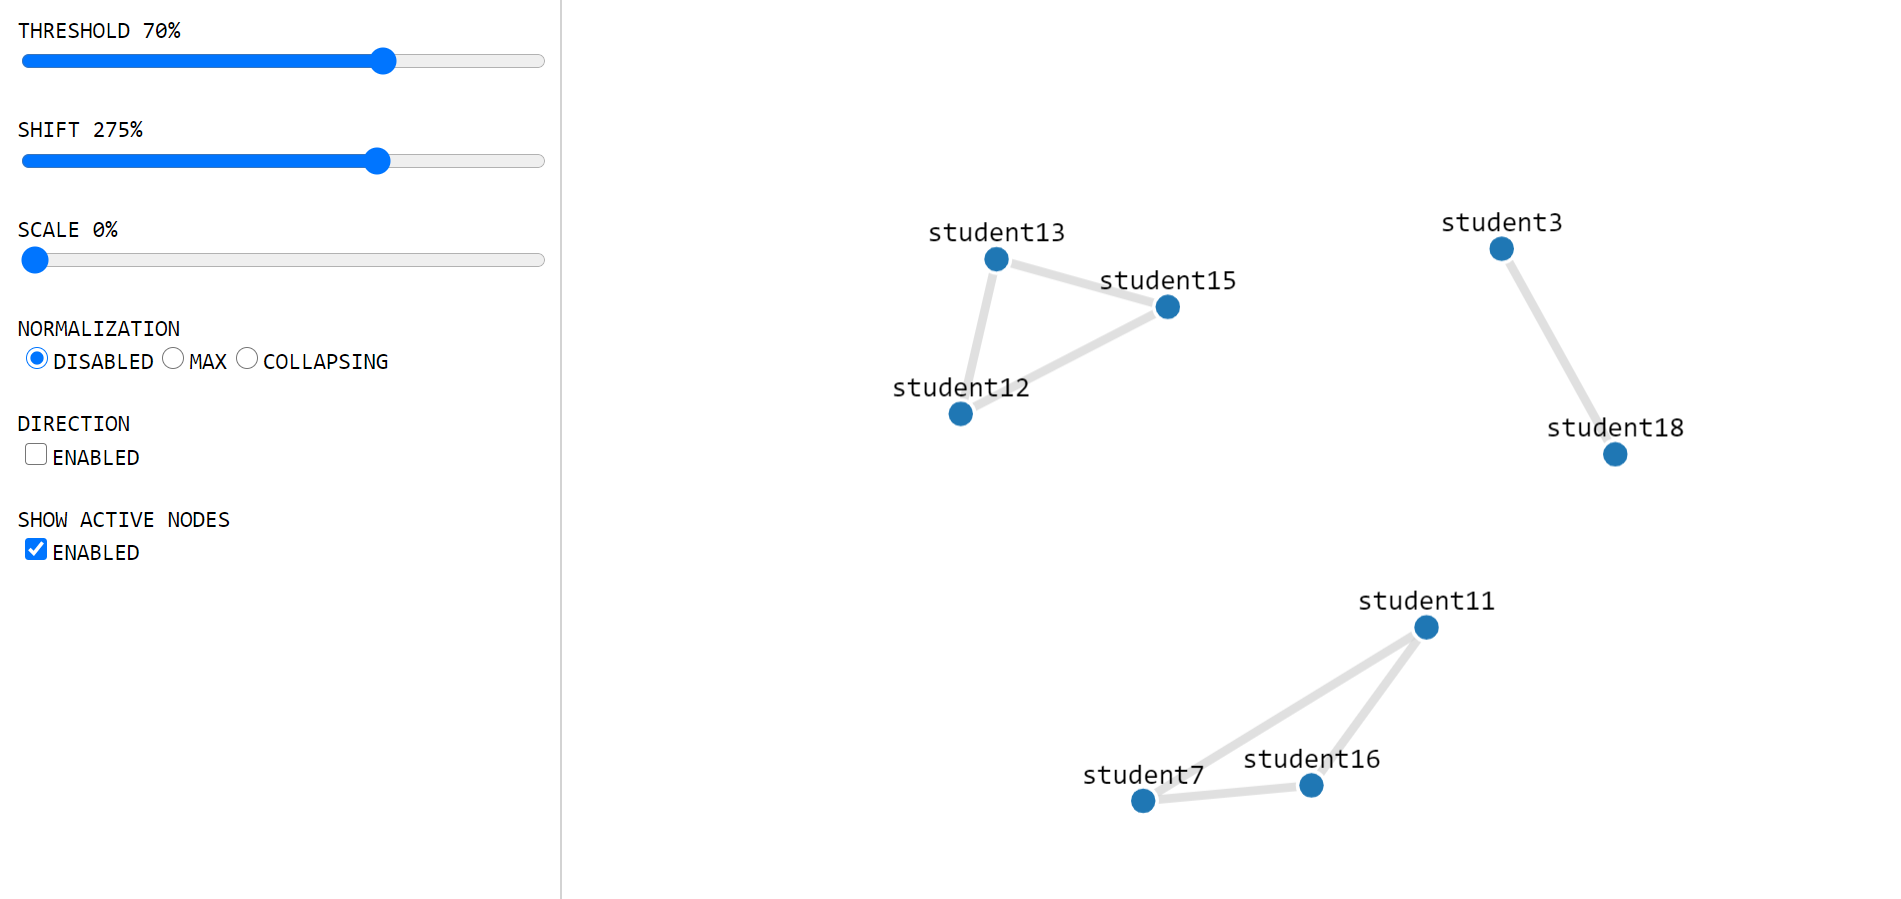
\includegraphics[width=1.0\textwidth]{graph.png}
\caption{Граф заимствований}
\label{fig:graph}
\end{figure}

\subsection{Детальные отчеты}

Ручная проверка заимствований является неотъемлемым элементом исследования результатов анализа плагиата. В качестве отображения найденных заимствований приводятся попарные листинги связанных решений с цветовым выделением заимствованных участков. На рис. \ref{fig:diff} можно наблюдать пример отображения найденного заимствования. Заметно, что связанные решения отличаются несколькими простыми операциями рефакторинга.

\begin{figure}[h!]
\centering
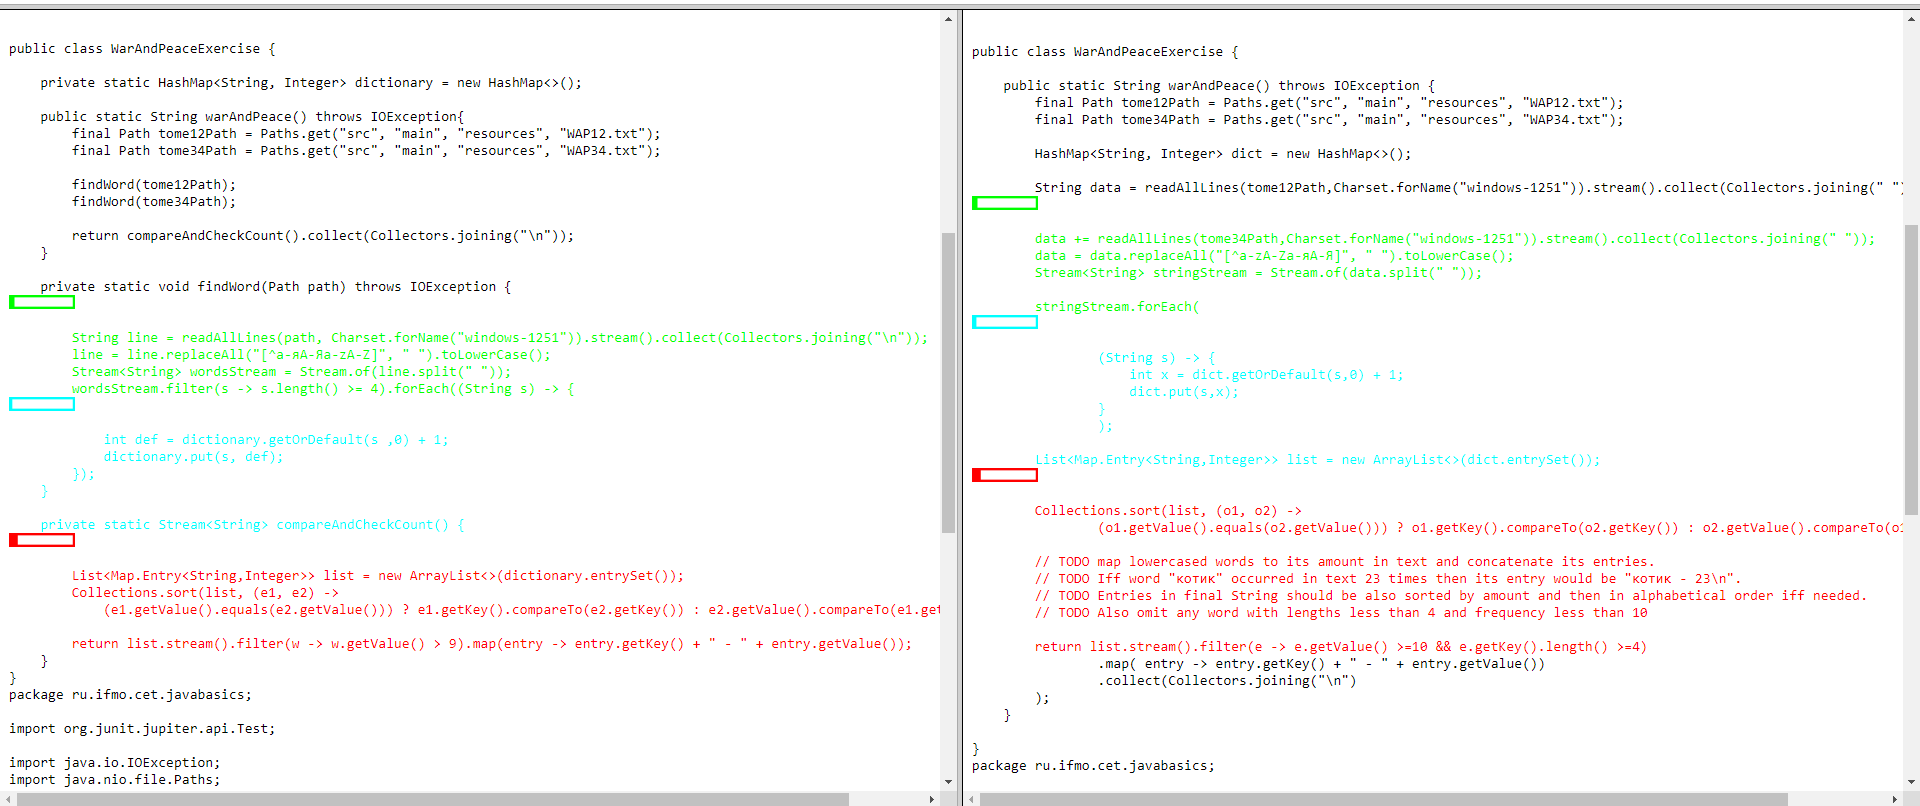
\includegraphics[width=1.0\textwidth]{plagiarism_match.png}
\caption{Детальное отображение заимствований}
\label{fig:diff}
\end{figure}

\section{Процесс анализа плагиата}

Целостное представление модуля анализа плагиата, описанного в настоящей работе, схематически представлено на рис. \ref{fig:pipeline}. Как можно увидеть, построенный процесс анализа плагиата решений обучающихся в рамках практических курсов по программированию включает в себя следующие шаги:

\begin{enumerate}
    \item агрегацию задания и решений,
    \item загрузку задания и решений на сервер MOSS,
    \item выгрузку всех результатов, сгенерированных MOSS,
    \item составление отчета по результатам анализа плагиата,
    \item генерирование графа заимствований.
\end{enumerate}

\begin{figure}[h!]
\centering
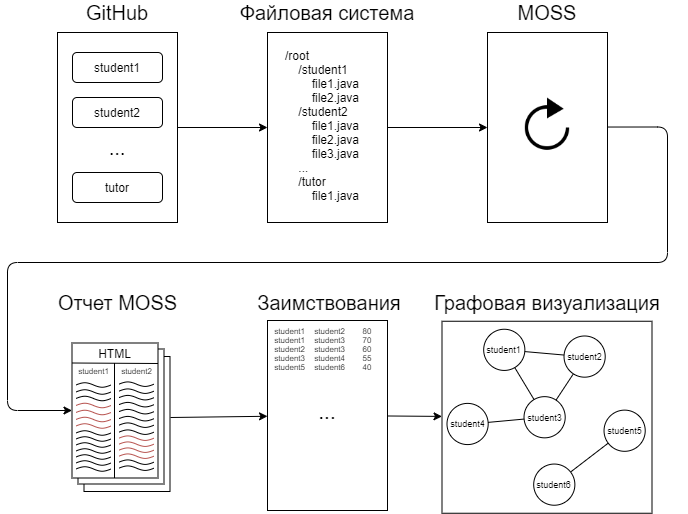
\includegraphics[width=1.0\textwidth]{plagiarism_pipeline.png}
\caption{Стадии анализа плагиата}
\label{fig:pipeline}
\end{figure}

Результатом работы построенного процесса являются адаптированные результаты анализа плагиата, которые можно исследовать несколькими способами, в том числе используя сводные таблицы результатов, интерактивный инструмент графовой визуализации, а также детальные отчеты для каждого из найденных заимствований.

\section{Дальнейшее развитие}

Представленный модуль анализа плагиата применялся на протяжении последних 4 семестров для проведения 10 практических курсов по программированию со средней численностью обучающихся порядка 40 человек, общим числом заданий порядка 50 и числом решений больше 2200. Как показала практика применения, модуль обладает значительным потенциалом с точки зрения наглядности представления результатов анализа плагиата и может быть использован для любых практических курсов по программированию сравнимого размера.

Тем не менее, построенный процесс анализа плагиата обладает рядом ограничений. Во-первых, визуализация на текущий момент учитывает данные об анализе плагиата только одного единственного задания. При этом, как было отмечено ранее в настоящей работе, наложение результатов анализа плагиата нескольких заданий положительно влияет на общее качество визуализации. Во-вторых, на текущий момент визуализация результатов анализа плагиата представляется лишь одним из возможных подходов - графовым отображением. Однако, поддержка иных видов визуализации может улучшить наглядность результатов работы модуля анализа плагиата в целом.

\section{Заключение}

Построенный процесс анализа плагиата для практических курсов по программированию с использованием разработанного инструмента графовой визуализации позволяет отвечать на новые вызовы в современном образовании, появляющиеся в связи с активным развитием электронного обучения, массового образования и связанных с ними автоматизированных инструментов контроля результатов обучения.

При этом крайне важно понимать, что никакой автоматизированный процесс анализа плагиата не дает результатов, которые можно было бы слепо использовать для выделения недобросовестных обучающихся. Каждый отдельный случай должен индивидуально исследоваться преподавателем. Стоит также отметить, что проблемой могут быть не только заимствования, но и риск представления оригинального, но не самостоятельно написанного решения. Именно поэтому в системе Flaxo результаты всех автоматизированных проверок используются лишь в качестве рекомендаций, а ключевые решения об оценивании решений обучающихся осуществляются преподавателем, в том числе после очного собеседования.

Описанный ранее процесс значительно упрощает проведение анализа плагиата и интерпретацию его результатов. В итоге, преподаватель имеет возможность интерактивно изучать все автоматически найденные заимствования и эффективно классифицировать решения обучающихся, как оригинальные и заимствованные.

\bibliographystyle{plain}
\bibliography{references}
\end{document}
